Software ist verschiedenartig verbreitet und kann verschiedene Eigenschaften aufweisen, die sich oftmals mit Merkmalen anderer Softwarevarianten decken und daher nicht leicht voneinander zu unterscheiden sind. \cite[S. 3]{wichmann_linux-_2005}

\begin{figure}[h]
    \centering
    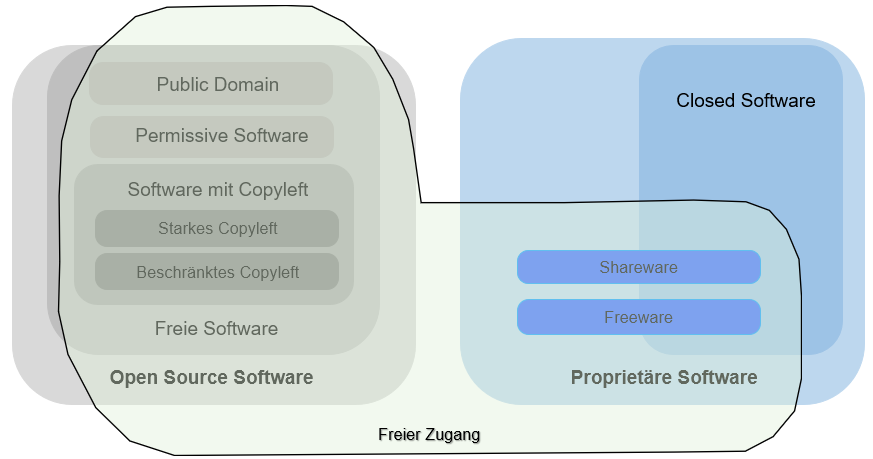
\includegraphics[scale=0.6]{Bilder/AbgrenzungSWvarianten.png}
    \caption{Abgrenzung der unterschiedlichen Softwarevarianten, \cite[S. 7]{wichmann_linux-_2005}}
\end{figure}

In diesem Fall müssen die wesentlichen Eigenschaften der unterschiedlichen Varianten herausgearbeitet werden, damit eine Abgrenzung zu OSS stattfinden kann. Innerhalb der Abbildung 9 werden die wesentlichen Softwarevarianten und deren gemeinsame Schnittpunkte schematisch dargestellt und im folgenden Kapitelteil übersichthaft kurz vorgestellt. 

\paragraph{2.2.2.1. Software} $~$

Unter Software versteht man ein immatrielles Produkt, welches zunächst durch das Urherberrecht geschützt ist. \cite[S. 24]{groll_1x1_2021} Der geschriebene Quellcode wird durch die Kompilierung in ein lauffähiges Programm ausgeführt.

\paragraph{2.2.2.2. Freie Software}$~$

Freie Software oder Free Software liegt vor, wenn der Quellcode frei zugänglich ist, modifiziert und weiterverbreitet werden kann. Nutzer können die Software zwar nach ihren persönlichen Vorstellungen und Anforderungen individualisieren, jedoch fallen die Modifikationen bei der Weitergabe der Software unter dieselben Lizenzbedingungen wie die ursprüngliche Software. \cite{fsf_freie_3021} Obwohl freie Software oftmals als ein Synonym zu OSS verwendet wird und viele Paralellitäten aufweist, entspricht dies nicht der Tatsache. Freie Sofware ist von Richard Stallman geprägt worden und beschreibt ein gesellschaftliches Ideal zur grenzenlosen Übermittlung von Wissen. \cite[S. 5]{wichmann_linux-_2005} Nutzer sollen frei und unabhängig von großen Softwareherstellern Software modifizieren und weiterverbreiten können. Die freie Software wurde durch die FSF definiert und beschreibt vier wesentliche Freiheiten \cite{fsf_freie_3021} die den Nutzern eingeräumt werden und in diesem Zusammenhang gelten müssen: 

\begin{itemize}
    \item Freiheit, das Programm für jeden Zweck zu nutzen
    \item Freiheit, das Programm nach der Funktionsweise zu untersuchen und nach den eigenen Bedürfnissen anzupassen
    \item Freiheit, die Software zu kopieren und zu verteilen
    \item Freiheit, das Programm zu verbessern und diese weiterzugeben
\end{itemize}

Im Ergebnis ist freie Software stehts OSS, allerdings handelt es sich nicht bei jeder OSS um eine freie Software. \cite[S. 28]{kees_open_2015}

\paragraph{2.2.2.3. Open Source}$~$

Ähnlich zu freier Software handelt es sich bei OSS um eine Software, dessen Quellcode frei zugänglich ist, modifiziert und weiterverbreitet werden kann. Der Nutzer erhält damit Nutzungsrechte an der Software durch den Lizenzgeber. Wesentlicher Unterschied zu freier Software besteht darin, dass der Fokus von OSS im Hinblick auf den Zugang zum Quellcode rein praktischer Natur ist, während freie Software den Zugang auf eine ethische und soziale Ebene abstellt. \cite[S. 28]{kees_open_2015} Kernelement von freier als auch von OS-Software ist die freie Verfügbarkeit des Quellcodes, um die Entwicklung von qualitativ hochwertiger, zuverlässiger und flexibler Software voranzutreiben. Basierend auf diesem Grundgedanken der OSI wurde die Lizenz von 'Open-Source' als eine Gruppe von mehreren Kritierien \cite{open_source_inititative_open_2018} definiert, die erfüllt werden müssen. Bei diesen Kritierien handelt es sich nicht um eine Lizenz von Open-Source, sondern um einen Standard an dem die Lizenzen von OSS gemessen werden können und insbesondere die die Bedingungen für die Verbreitung und Weitergabe der Software regeln. 

\begin{itemize}
    \item \textit{Freie Weitergabe}\\
    Die Lizenz darf niemanden daran hindern, die Software als Bestandteil eines gesamten Softwarepaktes, dessen Programme aus unterschiedlichen Quellen basieren, zu verkaufen oder weiterzugeben. Zudem dürfen keine Lizenz- oder sonstige Gebühren für diesen Fall verlangt werden. 

    \item \textit{Quellcode}\\
    Das Programm muss zwingend einen Quellcode enthalten und die Weitergabe in kompilierter Form ermöglichen. Sollte eine Weitergabe des Programms ohne Quellcode erfolgen, so muss eine Möglichkeit geschaffen werden, den Quellcode kostenlos aus dem Internet herunterzuladen. Hierbei muss der Quellcode verständlich und veränderbar sein. 

    \item \textit{Abgeleitete Software}\\
    Die Lizenz muss Modifikationen und deren Weitergabe unter denselben Bedingungen erlauben wie die Lizenz der ursprünglichen Software. 

    \item \textit{Unversehrheit des Quellcodes des Autors}\\
    Innerhalb der Weitergabe des modifizierten Quellcodes, müssen zusätzlich 'Patch-Files' weitergegeben werden, in denen festgelegt ist, welche Autoren bei der Entwicklung beteiligt waren. Darüber hinaus muss die Weitergabe der Software, basierend auf dem veränderten Quellcode, ausdrücklich erlaubt sein. 

    \item \textit{Keine Diskriminierung von Personen und Gruppen}\\
    Keine Benachteiligung durch die Lizenz.
    
    \item \textit{Keine Einschränkung bezüglich des Einsatzfeldes}\\
    Keine Beschränkung der Lizenz aufgrund eines Einsatzgebietes  

    \item \textit{Weitergabe der Lizenz}\\
    Die verbundenen Rechte des Programmes müssen bei einer Weitergabe für alle gelten, ohne dass eine zusätzliche Lizenz für die betreffenden Parteien anfällt. Dies gilt insbesondere für das späte Hinzufügen von Klauseln. 

    \item \textit{Die Lizenz darf nicht auf ein bestimmtes Produktpaket beschränkt sein}\\
    Die Rechte eines Programmteils dürfen nicht von einem bestimmten Softwarepaket abhängig sein. Sollten einzelne Programmteile weitergegeben werden, so gilt die gleiche Lizenz, die auch innerhalb des ursprünglichen Softwarepaket gewährt wurde.

    \item \textit{Die Lizenz darf die Weitergabe zusammen mit anderer Software nicht einschränken}\\
    Es darf keine Einschränkung anderer Software durch die entsprechende Lizenz eines Programmes geben.

    \item \textit{Die Lizenz muss technologieneutral sein}\\
    Die Lizenz darf keine bestimmte Schnittstelle, individuelle Technologie oder Softwarearten ausschließen. 

\end{itemize}

\paragraph{2.2.2.4. Proprietäre Software}$~$

Proprietäre Software bezeichnet Software die "urheberrechlich geschützt" ist und folglich der Urheber, meist ein Unternehmen, die alleinige Entscheidungsgewalt über den Umgang mit der entsprechenden Software hat. \cite[S. 26]{groll_1x1_2021} In diesem Rahmen ist der Quellcode nicht frei zugänglich, wodurch die technische Analyse nicht möglich ist. \cite[S. 15]{wilmer_rechtliche_2021} Auch die Weiterverbreitung oder Modifikation ist verboten und bedarf ausschließlich die Erlaubnis des Rechtsinhabers. Damit sollen wichtige Entwicklungen, Implementierungen von Schnittstellen oder Algorithmen umfassend geschützt werden. Oftmals wird beim Kauf einer proprietären Software, lediglich ein zeitlich begrenztes Nutzungsrecht und kein dauerhaftes Eigentumsrecht eingeräumt. \cite[S. 15]{wilmer_rechtliche_2021} Folglich kann die bereits kompilierte Software ausschließlich installiert oder ausgeführt werden. 

\paragraph{2.2.2.5. Kommerzielle Software}$~$

Ähnlich zu proprietären Software verfolgt kommerzielle Software das Ziel, Gewinn zu erwirtschaften. \cite[S. 14]{bitkom_ev_open_2016} Die Entwicklung als auch die Weitergabe erfolgt durch Entwickler innerhalb eines Unternehmens, wodurch der Quellcode nicht frei zugänglich ist und das Recht auf Weiterverbreitung oder Modifikation nicht gewährt wird. Obwohl kommerzielle und proprietäre Software sich stark ähneln, sind kommerzielle Software selten kostenlos erhältlich aber machen den wesentlichen Unterschied aus. \cite[S. 4]{wichmann_linux-_2005}

\paragraph{2.2.2.6. Public Domain}$~$

Public Domain Software beschreibt einen fehlenden oder teilweise nicht vorhandenen Urheberrechtsschutz einer Software, aufgrund des Abtretens aller Rechte an die Allgemeinheit durch den Urheber. \cite[S. 14]{renner_open_2006} Durch den Verzicht des Urheberrechts des Autors kann der Nutzer die Software uneingeschränkt verwenden, kopieren und verteilen. Allerdings muss der Quellcode bei Public Domain im Vergleich zu OSS nicht frei zugänglich sein. \cite[S. 14]{renner_open_2006}  Während dem Lizenznehmer innerhalb der OSS Veränderungs- und Weiterverbreitungsrechte basierend auf dem Urheberrecht eingeräumt werden, verzichtet der Autor einer Public Domain darauf und zeigt den wesentlichen Unterschied zu OSS auf. \cite[S. 10]{wilmer_rechtliche_2021} Public Domain Software ist allerdings im angloamerikansichen Raum bekannt. Nach deutschen Recht ist der Verzicht aller Urheberrechte nicht möglich, weshalb lediglich eine Einräumung eines Nutzungsrechtes vorliegt, die dem Lizenznehmer die unbeschränkte Verwertung gewährt allerdings die Urheberpersönlichkeitsreche unberührt lässt. \cite[S. 14]{renner_open_2006}

\paragraph{2.2.2.7. Shareware}$~$

Grundsätzlich kann der Nutzer ein Softwareprdukt, basierend auf einer Shareware kostenlos verbreiten, kopieren und testen, wobei die volle Funktionsfähigkeit nur auf einen bestimmten Zeitraum beschränkt ist. \cite[S. 27]{groll_1x1_2021} Will der Nutzer die Software über den bestimmten Testzeitraum nutzen, müssen bestimmte Lizenzgebüren errichtet werden. Shareware eignet sich besonders um Software vor einem endgültigen Kauf zu testen. \cite[S. 14/15]{renner_open_2006} Überdies entspricht Shareware im Wesentlichen einer proprietären Software.

\paragraph{2.2.2.8. Freeware}$~$

Freeware entspricht einer Software, dessen Urheber ein kostenloses Nutzungs- und Weiterverbreitungsrecht einräumt.\cite[S. 26]{groll_1x1_2021} Da der Quellcode für diese Softwareart nicht einsehbar ist, ist im Gegensatz zu OSS eine Modifikation der Software nicht möglich. Ferner hat der Autor die Möglichkeit, die Lizenzbestimmungen beliebig aufzustellen und zu verändern. \cite[S. 14]{renner_open_2006} Während die Nutzung im kommerziellen Gebrauch zu weiteren Lizenzgebüren führen, ist Freeware im privaten Gebrauch kostenlos zulässig.\\

\newcommand\T{\rule{0pt}{4ex}}
\newcommand\B{\rule[-3ex]{0pt}{0pt}}

\begin{table}
    \begin{center}
        \begin{tabular}[h]{|r|c|c|c|c|}
        \hline\hline
        \T\parbox{3cm}{SW-Varianten} & \parbox{2.5cm}{Unterliegt einer Lizenz} & Modifzierbar & Kostenlos & \parbox{2cm}{offener Quellcode} \B\\
        \hline\hline
        \parbox{3cm}{Freie Software} & \checkmark & \checkmark & \checkmark & \checkmark \\
        \hline
        \parbox{3cm}{Open Source} & \checkmark & \checkmark & \checkmark & \checkmark  \\
        \hline
        \T\parbox{3cm}{Proprietäre Software} & \checkmark & \xmark & \xmark & \xmark \B \\
        \hline
        \T\parbox{3cm}{Kommerzielle Software} & \checkmark & \xmark & Selten & \xmark \B \\
        \hline
        \parbox{3cm}{Public Domain} & \xmark &  \xmark & \checkmark & \xmark  \\
        \hline
        \parbox{3cm}{Shareware} & \checkmark & \xmark & \xmark & \xmark \\
        \hline
        \parbox{3cm}{Freeware} & \checkmark & \xmark & \checkmark & \xmark  \\
        \hline
        \end{tabular}
    \caption{Gängige Softwarevarianten im Vergleich, angelehnt an \cite[S. 9]{wilmer_rechtliche_2021}, \cite[S. 28]{groll_1x1_2021}}
    \end{center}
\end{table}
   
Anhand der vorliegenden Tabelle 1 lassen sich die Unterschiede in den Katergorien Lizenz, Veränderbarkeit, Preis und freier Zugang voneinander unterscheiden. 


